% Filled shapes and straight lines in TikZ pictures, and their labels under a
% rotation, a scale and a mirror. A picture's straight strokes and
% four-cornered fills (arrow tips among them) are the shapes a rule is, and
% count as rules on both sides; a stroked outline, a curve or a triangle on
% neither. At 11pt, labels at \normalsize and \small use one font at two
% sizes, and only the glyphs drawn are counted, not the outlines a picture
% keeps out of sight. The PDF draws the pictures as TeX
% does (tex_pictures).
\documentclass[11pt]{article}
\usepackage{tikz}
\begin{document}
A paragraph before the pictures, long enough to break across lines
differently at every width the test tries, so that each picture below
moves when the text is reflowed.

\begin{center}
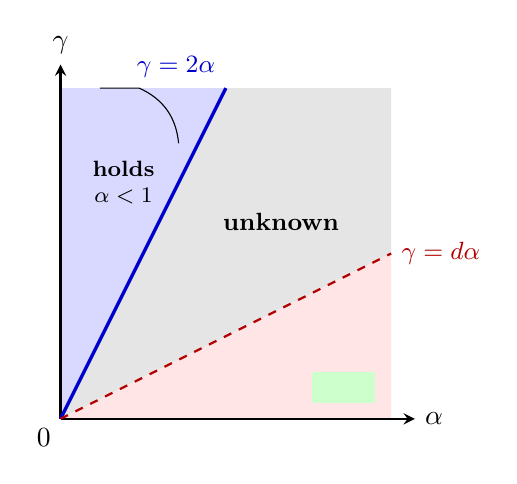
\begin{tikzpicture}
  \fill[blue!15] (0,0) -- (2.1,4.2) -- (0,4.2) -- cycle;
  \fill[gray!20] (0,0) -- (2.1,4.2) -- (4.2,4.2) -- (4.2,2.1) -- cycle;
  \fill[red!10] (0,0) -- (4.2,2.1) -- (4.2,0) -- cycle;
  \fill[green!20] (3.2,0.2) rectangle (4,0.6);
  \draw[->, >=stealth, thick] (0,0) -- (4.5,0) node[right] {$\alpha$};
  \draw[->, >=stealth, thick] (0,0) -- (0,4.5) node[above] {$\gamma$};
  \node[below left] at (0,0) {$0$};
  \draw[very thick, blue!80!black] (0,0) -- (2.1,4.2)
    node[above left, font=\small] {$\gamma = 2\alpha$};
  \draw[thick, dashed, red!70!black] (0,0) -- (4.2,2.1)
    node[right, font=\small] {$\gamma = d\alpha$};
  \draw (0.5,4.2) -- (1,4.2) to[bend left] (1.5,3.5);
  \node[align=center, font=\footnotesize] at (0.8,3.0) {\textbf{holds}\\ $\alpha<1$};
  \node[align=center, font=\small] at (2.8,2.5) {\textbf{unknown}};
\end{tikzpicture}
\end{center}
Text between two pictures, with a word or two more to fill the line.

\begin{center}
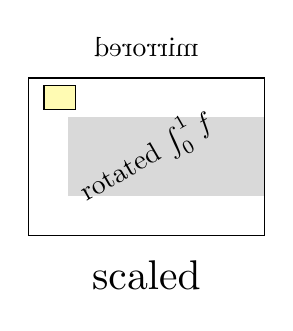
\begin{tikzpicture}
  \begin{scope}
    \clip (0,0) rectangle (3,2);
    \fill[gray!30] (0.5,0.5) rectangle (3.5,1.5);
  \end{scope}
  \draw (0,0) rectangle (3,2);
  \filldraw[fill=yellow!30] (0.2,1.6) rectangle (0.6,1.9);
  \node[rotate=30] at (1.5,1) {rotated $\int_0^1 f$};
  \node[scale=1.5] at (1.5,-0.5) {scaled};
  \node[xscale=-1] at (1.5,2.4) {mirrored};
\end{tikzpicture}
\qquad
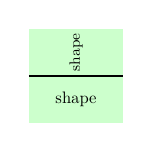
\begin{tikzpicture}[scale=0.6, every node/.style={transform shape}]
  \fill[green!20] (-1,-1) rectangle (1,1);
  \draw[thick] (-1,0) -- (1,0);
  \node[rotate=90, font=\small] at (0,0.5) {shape};
  \node at (0,-0.5) {shape};
\end{tikzpicture}
\end{center}
A last paragraph after the pictures.
\end{document}
